
\actTitle{Worksheet Problem Solving}

\noindent \textbf{Instructions:}  Work together in groups of  3 or 4 to complete the following problems.


\begin{enumerate}



\item The value of a newly purchased equipment is a linear function of time. A company purchases a piece of equipment for \$40,000. After 5 years, the equipment loses 15\% of its value. Answer the following:

\begin{enumerate}
\item Determine the value of the equipment after 5 years.
\item Express the value V (in dollars) of the equipment as a function of time t (in years) since purchase.
\item Determine the total time (in years) it will take for the machine to be worth 45\% of its original value.
\end{enumerate}

\vfill

\item Give the coordinates of all of the points that lie on \emph{both} the parabola $y=x^2+1$ \emph{and} the line $y=2x+4$.  Use the following steps to answer the question.
	\begin{enumerate}
		\item How can one describe an arbitrary point on the line $y=2x+4$ as an ordered pair?
		\item How can one describe an arbitrary point on the line $y=x^2+1$ as an ordered pair?
		\item How do these descriptions help you find the intersection.
	\end{enumerate}

\vfill
\newpage


\item You have 50 cm of wire, and you have to use part of this wire to
make a rectangle that's twice as long as it is wide, and the rest of the wire (if there
is any left) to make a square.
What should the dimensions of the shapes be if you want the total area to be as
small as possible? 

\newpage

\item Find the point $(x,y)$ lying on the parabola $y = x^2 + 2x + 1$ so that the average rate of change on the interval between $x$ and $2$ is zero.

\vfill

\item On the coordinate axes below, draw a function whose domain is
	$$[-2,1]\cup(2,3]\cup\{5\}$$
	and whose range is
	$$[-6,-4)\cup[-1,1]\cup\{2\}\cup(3,4].$$

\begin{center}
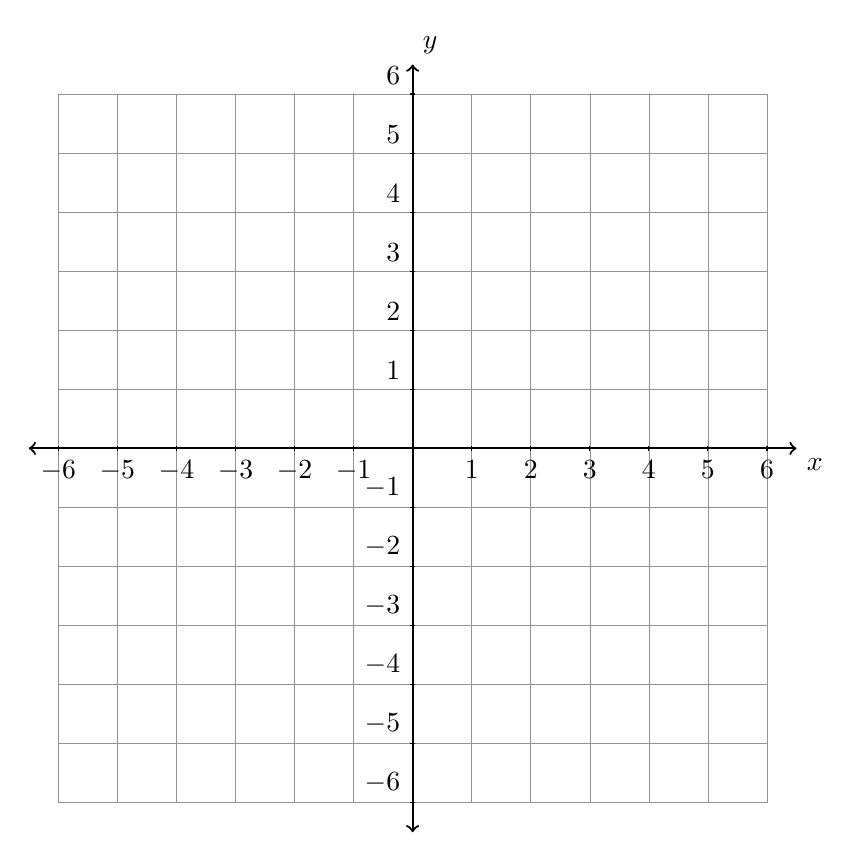
\begin{tikzpicture}[y=.75cm, x=.75cm,font=\sffamily,
	mydot/.style={
    circle,
    fill=white,
    draw,
    outer sep=0pt,
    inner sep=1.5pt
    }]
    %% Add a grid
    \draw[step = 1, gray, very thin,opacity=0.85] (-6, -6) grid ( 6, 6);
 	%% Draw the axes
	\draw[thick,<->] (-6.5,0) -- coordinate (x axis mid) (6.5,0) node[anchor = north west] {$x$};
    \draw[thick,<->] (0,-6.5) -- coordinate (y axis mid) (0,6.5) node[anchor = south west] {$y$};
    %% Label the y axis
    \foreach \y in {-6,...,-1,1,2,...,6} {
    	\draw (1pt, \y) -- (-1pt, \y) node[anchor = south east] {$\y$};
    }
    %% Label the x axis
    \foreach \x in {-6,...,-1,1,2,...,6} {
    	\draw (\x,1pt) -- (\x,-1pt) node[anchor = north] {$\x$};
    }
    %% Draw the function.
%    \begin{scope}
%         \draw[scale=1.0,very thick,black] (-2, 0) -- (1,-2);
%         \draw[scale=1.0,very thick,black] (1.05,1.04) -- (3,2);
%         \fill[black] (-2, 0) circle[radius=0.5ex];
%         \fill[black] (3,2) circle[radius=0.5ex];
%         \fill[black] (1,-2) circle[radius=0.5ex];
%         \draw[scale=1.0, very thick, black] (1,1) circle[radius=0.5ex];
%    \end{scope}

    %%\node[above=0.1cm] at (-2,2 )   {\nextXValue};

\end{tikzpicture}
\end{center}




\newpage

\item Find the point $P$ on the graph of $\sqrt{x}$ such that the line through $P$ and $(1,1)$ has slope $\displaystyle \frac{4}{7}$.
\vfill




\item A business forms a model of its widget sales via a pricing function $p(x) = 400-\frac{70}{8}x$. Here, $x$ is the number of widgets sold and $p(x)$ is the sales price in dollars per widget.  
\begin{enumerate}
\item Find the revenue function $R(x)$ for this business (revenue is total sales). 
\item Find the number $x$ sold that will maximize revenue. (This will be an unrealistic fraction,
but do not round.)
\item What is the maximum revenue? 
\item What is the price $p(x)$ that yields maximum revenue?
\end{enumerate}

\vfill
\vfill



%\newpage
%
%
%\newpage
%
%\item A small business makes scarves and sells them at the farmer's market.  The fixed monthly cost for the rental space at the farmer's market is \$200.  The cost of labor and supplies for the scarves amounts to \$7 per scarf, which are sold for \$35 each at the market.
%\begin{enumerate}
%\item Write a linear functions for the cost $C(x)$, revenue $R(x)$, and profit $P(x)$ corresponding to the production/sale of $x$ scarves per month.
%\vfill
%\item Determine the cost, revenue, and profit associated with selling 15 scarves in one month. Will the business make a profit or lose money that month?
%\vfill
%\item Determine the least number of scarves that must be produced and sold for a monthly profit.  Your answer should be an appropriate whole number.

%\end{enumerate}
%
%\vfill


%\newpage
%
%
%\vfill
%
%\item A diverter at the end of a gutter spout is meant to direct water away from a house.  The homeowner makes the diverter from a rectangular piece of aluminum that is 20 inches long and 12 inches wide.  She makes two folds both parallel to the 20 inch side.  Each fold is a distance \(x\) inches away from the edge.  
%\begin{enumerate}
%\item Write the volume of water that can be carried through the diverter as a function of \(x\).
%\item What is the maximum volume of water that can be carried through the diverter?
%\end{enumerate}  
%
%\vfill





\end{enumerate}


